\documentclass[UTF8,a4paper,10pt]{ctexart}
\usepackage[left=2.50cm, right=2.50cm, top=2.50cm, bottom=2.50cm]{geometry}
%页边距
\CTEXsetup[format={\Large\bfseries}]{section} %设置章标题居左

%%%%%%%%%%%%%%%%%%%%%%%
% -- text font --
% compile using Xelatex
%%%%%%%%%%%%%%%%%%%%%%%
% -- 中文字体 --
%\setmainfont{Microsoft YaHei}  % 微软雅黑
%\setmainfont{YouYuan}  % 幼圆    
%\setmainfont{NSimSun}  % 新宋体
%\setmainfont{KaiTi}    % 楷体
%\setmainfont{SimSun}   % 宋体
%\setmainfont{SimHei}   % 黑体
% -- 英文字体 --
%\usepackage{times}
%\usepackage{mathpazo}
%\usepackage{fourier}
%\usepackage{charter}

%\usepackage{helvet}

\usepackage{amsmath, amsfonts, amssymb} % math equations, symbols
\usepackage[english]{babel}
\usepackage{color}	% color content
\usepackage{graphicx}	% import figures
\usepackage{url}	% hyperlinks
\usepackage{bm} 	% bold type for equations
\usepackage{multirow}
\usepackage{booktabs}
\usepackage{epstopdf}
\usepackage{epsfig}
\usepackage{algorithm}
\usepackage{algorithmic}
\usepackage{listings}
\usepackage{xcolor}
\usepackage{booktabs}
\usepackage{zhnumber}
\usepackage{longtable}
\usepackage{subfigure}
\usepackage{float}
\usepackage{caption}
\usepackage{subfigure}
\renewcommand\thesection{\zhnum{section}}
\renewcommand \thesubsection {\arabic{section}}
\renewcommand{\algorithmicrequire}{ \textbf{Input:}}
% use Input in the format of Algorithm  
\renewcommand{\algorithmicensure}{ \textbf{Initialize:}}
% use Initialize in the format of Algorithm  
\renewcommand{\algorithmicreturn}{ \textbf{Output:}}
% use Output in the format of Algorithm  
%%%%%%%%%%%%%%%%%%
\usepackage{listings}
\usepackage{color}
\definecolor{dkgreen}{rgb}{0,0.6,0}
\definecolor{gray}{rgb}{0.5,0.5,0.5}
\definecolor{mauve}{rgb}{0.58,0,0.82}
\lstset{frame=tb,
  language=Python,
  aboveskip=3mm,
  belowskip=3mm,
  showstringspaces=false,
  columns=flexible,
  basicstyle={\small\ttfamily},
  numbers=left,%设置行号位置none不显示行号
  %numberstyle=\tiny\courier, %设置行号大小
  numberstyle=\tiny\color{gray},
  keywordstyle=\color{blue},
  commentstyle=\color{dkgreen},
  stringstyle=\color{mauve},
  breaklines=true,
  breakatwhitespace=true,
  escapeinside=``,%逃逸字符(1左面的键),用于显示中文例如在代码中`中文...`
  tabsize=4,
  extendedchars=false %解决代码跨页时,章节标题,页眉等汉字不显示的问题
}

%%%%%%%%%%%%%%%%%%%%%%%%%%%%
\usepackage{fancyhdr} %设置页眉、页脚
\pagestyle{fancy}
\lhead{}
\chead{}
%\rhead{\includegraphics[width=1.2cm]{fig/ZJU_BLUE.eps}}
\lfoot{}
\cfoot{}
\rfoot{}
\fancyfoot[RE,RO]{~\thepage~}

\fancyhead[RE,RO]{计算物理导论 \quad 2022春季学期 \quad 作业11 \quad 何翼成}

%%%%%%%%%%%%%%%%%%%%%%%
%  设置水印
%%%%%%%%%%%%%%%%%%%%%%%
%\usepackage{draftwatermark}         % 所有页加水印
%\usepackage[firstpage]{draftwatermark} % 只有第一页加水印
% \SetWatermarkText{Water-Mark}           % 设置水印内容
% \SetWatermarkText{\includegraphics{fig/ZJDX-WaterMark.eps}}         % 设置水印logo
% \SetWatermarkLightness{0.9}             % 设置水印透明度 0-1
% \SetWatermarkScale{1}                   % 设置水印大小 0-1    

\usepackage{hyperref} %bookmarks
\hypersetup{colorlinks, bookmarks, unicode} %unicode

\title{\textbf{矩阵对角化}}
\author{ 何翼成 \thanks{学号:520072910043; \newline
    邮箱地址:heyicheng@sjtu. edu. cn} }
\date{\today}

\begin{document}
\maketitle

%\begin{abstract}
%这是一篇中文小论文。这个部分用来写摘要。摘要的章标题默认是英文,还没找到改成中文的方法:(
%\end{abstract}
\section*{Project 1}
\section{题目分析}
%%%以下为插入图片模板
%\quad \newline
	\begin{figure}[!htbp]
		\centering
		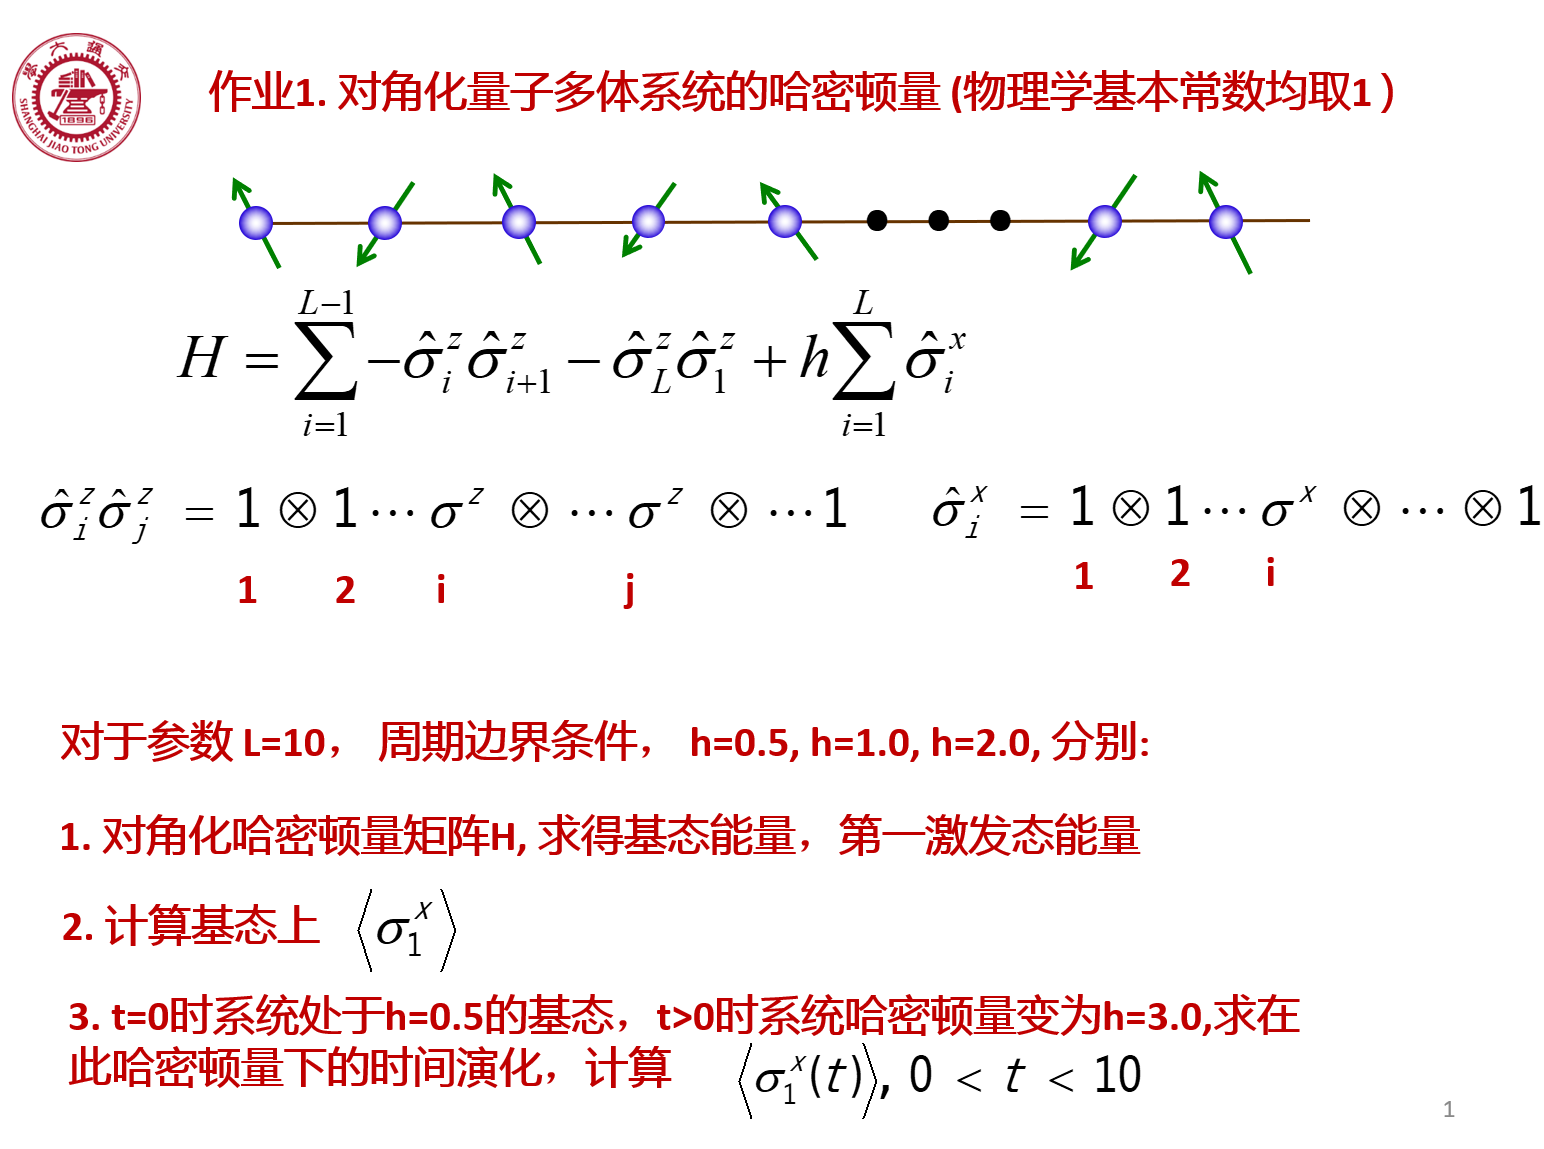
\includegraphics[width=1\textwidth,height=0.6\textwidth]{pictures/pro.png}
		\caption{题目总览} \label{project1}
	\end{figure}



\section{代码展示}
\lstset{language=matlab}
\begin{lstlisting}
    clear;clc;
    L=10;
    h=[1/2,1,2];
    
    %计算不同h下的基态能量和第一激发态
    he1e2=zeros(length(h),3);
    for n=1:length(h)
        hn=h(n);
        H=G(hn,L);
        En=unique(eig(H));
        disp("h="+hn+"时,基态能量为"+En(1,1)+",第一激发态为"+En(2,1))
        he1e2(n,1)=hn;he1e2(n,2)=En(1,1);he1e2(n,3)=En(2,1);
    end
    
    %计算基态的sigma_{1}^x的期望值
    disp("-------------------------------------------------")
    sigma1x_s=zeros(1,length(h));
    for n=1:length(h)
        hn=h(n);
        H=G(hn,L);
        [V,D]=eig(H);%V是特征值的对角矩阵,D使得H=DVD^(-1)
                     %易知D是特征向量(列向量)组成的矩阵
        psi0=V(:,1);
        sigma1x=psi0'*Sigmax(1,L)*psi0;
        sigma1x_s(n)=sigma1x;
        disp("h="+hn+"时,sigma_{1}^2的期望值是"+sigma1x)
    end
    
    %t=0时系统处在h=0.5的基态,t>0时h=3,求哈密顿量的时间演化。
    disp("-------------------------------------------------")
    tspan=0:0.1:10;%时间范围
    h=0.5;H=G(h,L);[~,D]=eig(H);psi0=V(:,1);%计算初态波函数
    h=3;H=G(h,L);
    sigma1x_t=zeros(1,length(tspan));
    for n=1:length(tspan)
        t=tspan(n);
        psi=expm(-1i*H*t)*psi0;
        sigma1x=conj(psi.')*Sigmax(1,L)*psi;
        sigma1x_t(n)=sigma1x;
        clc;
        disp("已完成计算进度"+n/length(tspan)*100+"%")
    end
    plot(tspan,sigma1x_t,'k')
    xlabel("Time")
    ylabel("<\sigma_{1}^x>")
    
    %%
    %定义H的生成函数
    function H=G(h,L)
        H=0;
        for i=1:L-1
            H=H-Sigmaz(i,i+1,L)+h*Sigmax(i,L);
        end
        H=H-Sigmaz(L,1,L)+h*Sigmax(L,L);
    end
    
    %生成单一的\hat{sigma_{i}}^z \hat{sigma_{j}}^z元素,未求和
    function sigmaz=Sigmaz(i,j,L)
        sigmaZ=[1,0;0,-1];%定义元矩阵
        s=1;
        for n=1:L
            if n==i||n==j
                s=kron(s,sigmaZ);
            else
                s=kron(s,eye(2));
            end
        end
        sigmaz=s;
    end
    
    %生成单一的\hat{sigma_{i}}^x元素,未求和
    function sigmax=Sigmax(i,L)
        s=1;sigmaX=[0,1;1,0];%定义元矩阵
        for n=1:L
            if n==i
                s=kron(s,sigmaX);
            else
                s=kron(s,eye(2));
            end
        end
        sigmax=s;
    end
\end{lstlisting}

\section{结果分析与结论}
通过代入不同的初始量$h$,可以得到不同的结果。

\subsubsection{基态能量与第一激发态能量}
h=0.5时,基态能量为-10.6356,第一激发态为-10.6353\\
h=1时,基态能量为-12.7849,第一激发态为-12.6275\\
h=2时,基态能量为-21.2712,第一激发态为-19.2706\\
\quad \newline

\subsubsection{<sigma1x>}

h=0.5时,$\sigma_{1}^x$的期望值是-0.25897\\
h=1时,$\sigma_{1}^x$的期望值是-0.63925\\
h=2时,$\sigma_{1}^x$的期望值是-0.93408\\
\quad \newline

\subsubsection{哈密顿量的时间演化}

\begin{figure}[!htbp]
    \centering
    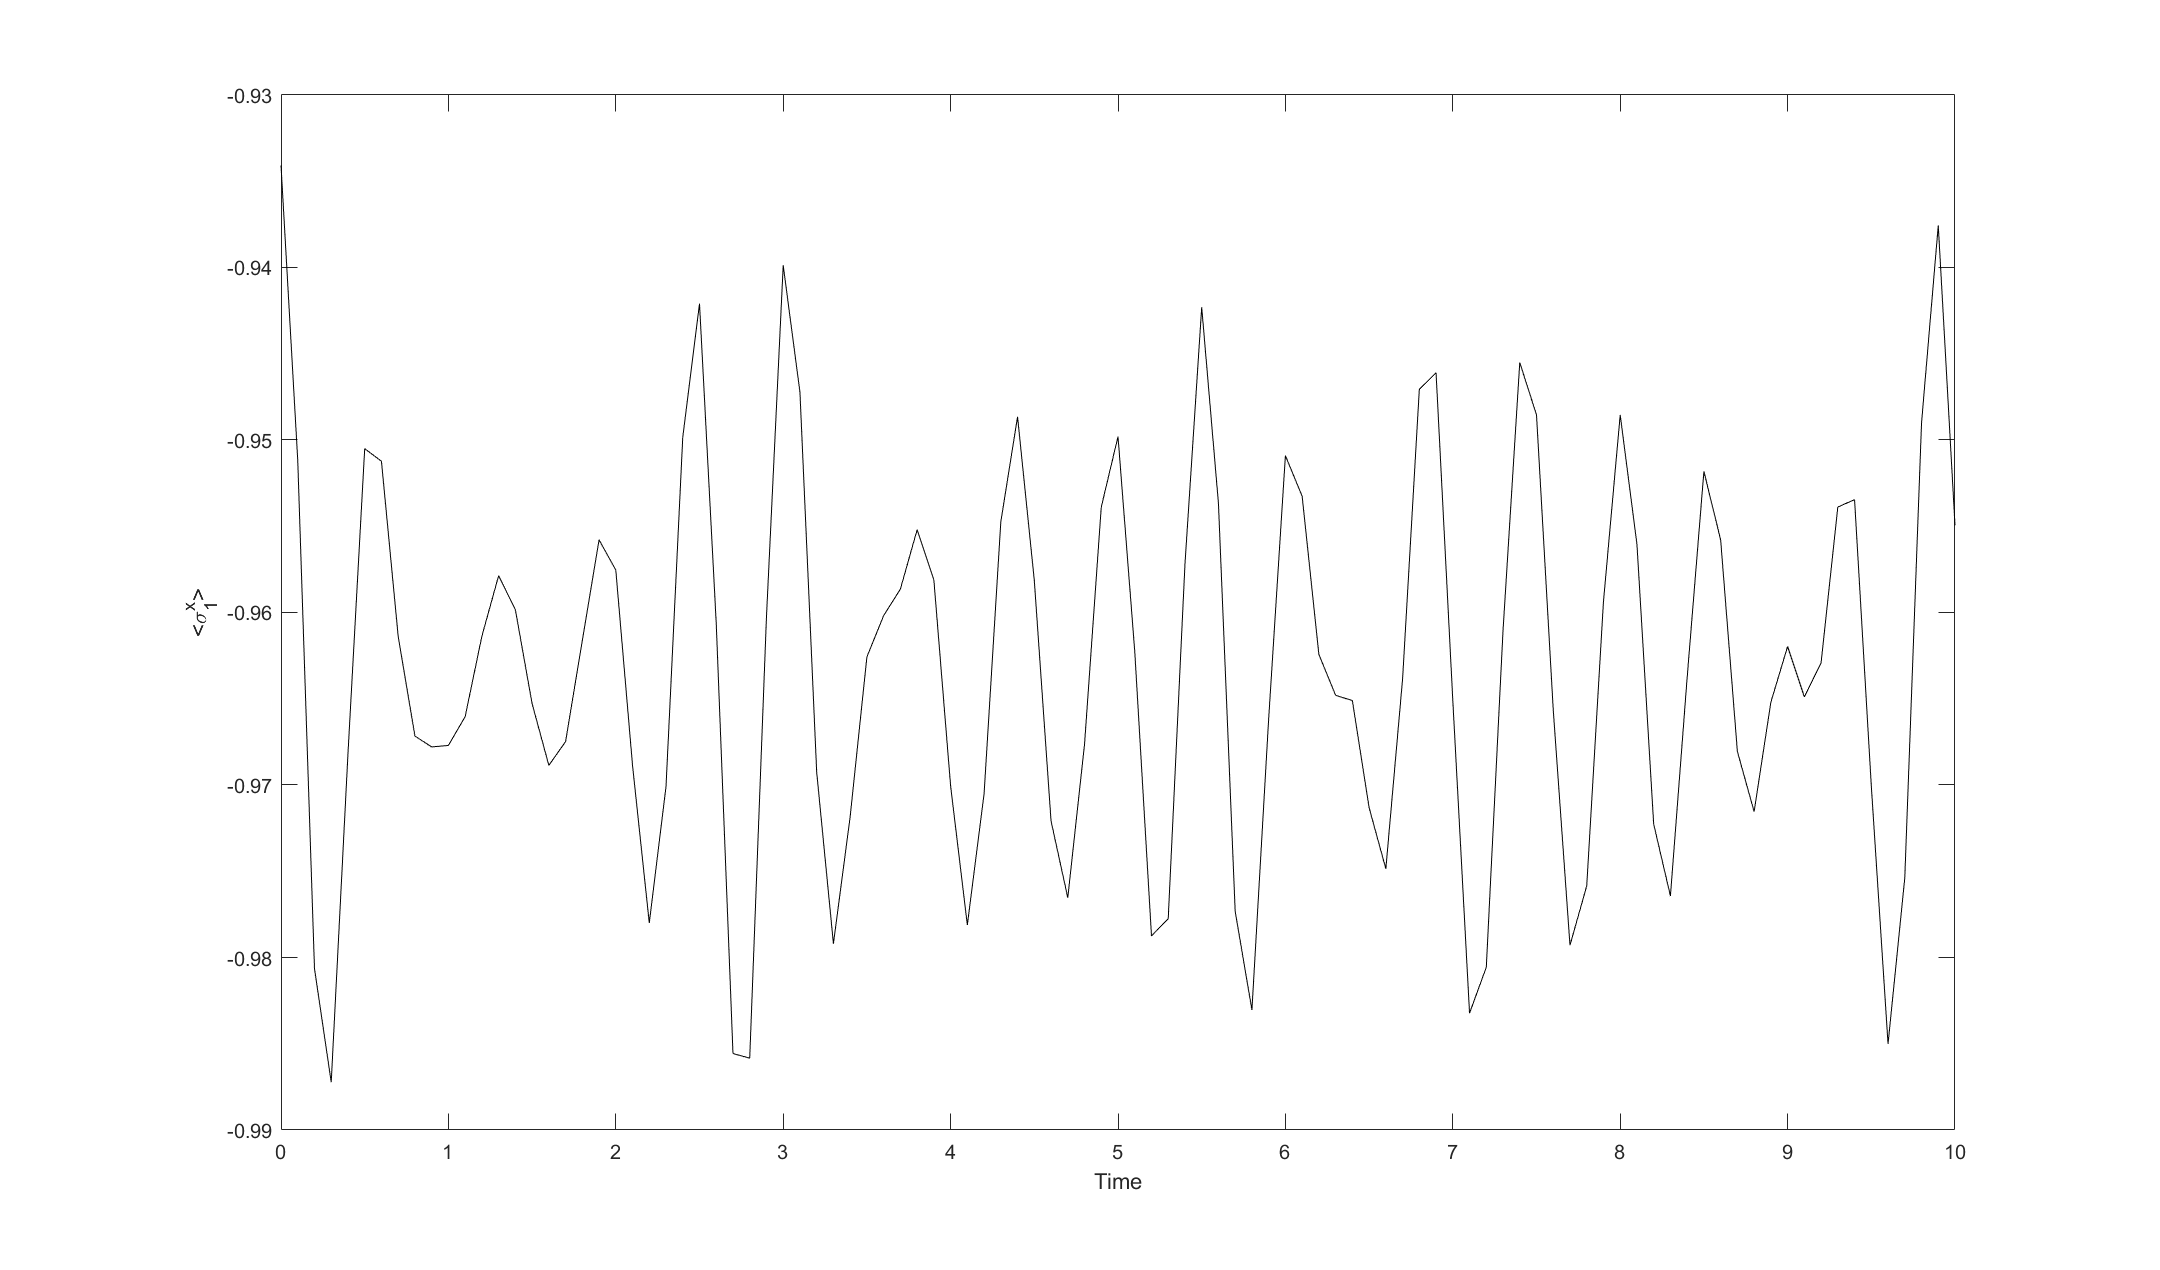
\includegraphics[width=1\textwidth,height=1\textwidth]{pictures/valuet.png}
    \caption{在[0,10]时间下的哈密顿量演化情况} \label{ek2}
\end{figure}

\section*{Project2}
  %%%%%%%%%%%%%%%%%%%%%%%%%第二题%%%%%%%%%%%%%%%%%%%%%%%%%%%%%%%%%
  %%%%%%%%%%%%%%%%%%%%%%%%%第二题%%%%%%%%%%%%%%%%%%%%%%%%%%%%%%%%%
  %%%%%%%%%%%%%%%%%%%%%%%%%第二题%%%%%%%%%%%%%%%%%%%%%%%%%%%%%%%%%
  %%%%%%%%%%%%%%%%%%%%%%%%%第二题%%%%%%%%%%%%%%%%%%%%%%%%%%%%%%%%%
  \section{解答}
  \subsubsection{1}
  \begin{equation}
      \begin{aligned}
          &H\psi=\lambda\psi\\
          &|H-\lambda I|=0\\
          &\Longrightarrow\lambda=\pm \sqrt{a^2+cc^{*}}\\
          &\text{代入不同的}\lambda\text{,即可求得不同的特征向量}\\
          &\lambda_{1}=\sqrt{a^2+cc^{*}}\Longrightarrow\psi_{1}=[c,\sqrt{a^2+cc^{*}}-a]\\
          &\lambda_{2}=-\sqrt{a^2+cc^{*}}\Longrightarrow\psi_{2}=[-c,\sqrt{a^2+cc^{*}}+a]
      \end{aligned}
  \end{equation}
%%%%%%%%%%%%%%%%%%%%%%%%%%%%%%%%%%%%%%%%%%%%%%%%%%%%%%%%%%%%%%%%%%%%%%%%%%%%%%%
  \subsubsection{2}
  \begin{equation}
      \begin{aligned}
          &\text{由矩阵对角化的性质可知,D即为对角元素为特征值的矩阵,而S为列向量为特征向量的矩阵。}\\
          &\text{可知}D=\textit{diag}\{\lambda_{1},\lambda_{2},\lambda_{3},\ddots\}\\
          &\text{而}S=[v_{1},v_{2},v_{3},\ddots],S^{-1}=[v_{1},v_{2},v_{3},\ddots]^{*},\text{其中}v_{i}\text{是对应}\lambda_{i}\text{的特征向量}\\
          &\text{由特征向量的正交不难知道其满足幺正矩阵的定义。}\\
          &\text{所以在本题中,若是代入第一问求得的值,可以得到:}\\
          &D=\left[
                \begin{array}{cc}
                \sqrt{a^2+cc^{*}} & 0\\\\
                0 & -\sqrt{a^2+cc^{*}}\\\\
                \end{array}
          \right]\\
          &S=\left[
                \begin{array}{cc}
                c/A & -c/B\\\\
                (\sqrt{a^2+cc^{*}}-a)/A & (\sqrt{a^2+cc^{*}}+a)/B \\\\
                \end{array}
          \right],\\
          &A=\sqrt{cc^{*}+(\sqrt{a^2+cc^{*}}-a))^2},B=\sqrt{cc^{*}+(\sqrt{a^2+cc^{*}}+a)^2},\\
          &\text{A,B是为了化为幺正矩阵而添加的系数}\\
      \end{aligned}
  \end{equation}
%%%%%%%%%%%%%%%%%%%%%%%%%%%%%%%%%%%%%%%%%%%%%%%%%%%%%%%%%%%%%%%%%%%%%%%%%%%%%%%
  \subsubsection{3}
  \begin{equation}
      \begin{aligned}
          &\text{已知}H=S^{-1}DS\\
          &e^{iHt}=e^{it(S^{-1}DS)}=\sum_{n=0}^{\infty}\frac{1}{n!}(it)^{n}(S^{-1}DS)^n\\
          &\text{而一般意义上,}(S^{-1}DS)*(S^{-1}DS)=S^{-1}D^2S,\text{所以}(S^{-1}DS)^n=S^{-1}D^nS\\
          &\text{所以}\sum_{n=0}^{\infty}\frac{1}{n!}(it)^{n}(S^{-1}DS)^n=S^{-1}[\sum_{n=0}^{\infty}\frac{1}{n!}(it)^{n}D^n]S\\
          &=S^{-1}e^{iDt}S\\
          &\text{同样的,对于}e^{iDt}\text{而言,即有}\\
          &e^{iDt}=\sum_{n=0}^{\infty}\frac{1}{n!}(it)^{n}D^n,\text{而对角矩阵}D=\textit{diag}\{\lambda_{1},\lambda_{2}\}\\
          &\text{对角矩阵拥有性质}D^n=\textit{diag}\{\lambda_{1}^n,\lambda_{2}^n\}\\
          &\text{所以有}\sum_{n=0}^{\infty}\frac{1}{n!}(it)^{n}D^n=\sum_{n=0}^{\infty}\frac{1}{n!}(it)^{n}\textit{diag}\{\lambda_{1}^n,\lambda_{2}^n\}\\
          &=\textit{diag}\{\sum_{n=0}^{\infty}\frac{1}{n!}(it)^{n}\lambda_{1}^n,\sum_{n=0}^{\infty}\frac{1}{n!}(it)^{n}\lambda_{2}^n\}\\
          &=\textit{diag}\{e^{i\lambda_{1}t},e^{i\lambda_{2}t}\}\\
          &\text{综上所述,},e^{iHt}=[v_{1},v_{2}]\textit{diag}\{e^{i\lambda_{1}t},e^{i\lambda_{2}t}\}[v_{1},v_{2}]^{T}\\
          &=e^{i\lambda_{1}t}v_{1}v_{1}^{T}+e^{i\lambda_{2}t}v_{2}v_{2}^{T}\\
          &=e^{i\lambda_{1}t}\left[
            \begin{array}{cc}
            cc^{*} &c\sqrt{a^2+cc^{*}}-ac \\\\
            c\sqrt{a^2+cc^{*}}-ac & 2a^2+cc^{*}-2a\sqrt{a^2+cc^{*}} \\\\
            \end{array}
      \right]/(cc^{*}+2a^2+cc^{*}-2a\sqrt{a^2+cc^{*}})\\
      &+e^{i\lambda_{2}t}\left[
        \begin{array}{cc}
        cc^{*} & -c\sqrt{a^2+cc^{*}}-ac\\\\
        -c\sqrt{a^2+cc^{*}}-ac & 2a^2+cc^{*}+2a\sqrt{a^2+cc^{*}} \\\\
        \end{array}
  \right]/(cc^{*}+2a^2+cc^{*}+2a\sqrt{a^2+cc^{*}})
      \end{aligned}
  \end{equation}
%以下为插入代码模板
%~\\
%\lstset{language=matlab}
%\begin{lstlisting}
%\end{lstlisting}


%%%以下为插入图片模板
%\quad \newline
%	\begin{figure}[!htbp]
%		\centering
%		\includegraphics[width=0.5\textwidth,height=0.375\textwidth]{pictures/minscale.png}
%		\caption{最小风向} \label{minsacle}
%	\end{figure}

%%%以下为插入图片模板
%\quad \newline
%	\begin{figure}[!htbp]
%		\centering
%		\includegraphics[width=0.5\textwidth,height=0.375\textwidth]{pictures/minscale.png}
%		\caption{最小风向} \label{minsacle}
%	\end{figure}

%    \begin{algorithm}
%		\caption{Title of the Algorithm}
%     	\begin{algorithmic}[1]
%			\REQUIRE some words.  % this command shows "Input"
%			\ENSURE ~\\           % this command shows "Initialized"
%			some text goes here ... \\
%			\WHILE {\emph{not converged}}
%			\STATE ... \\  % line number at left side
%			\ENDWHILE
%			\RETURN this is the lat part.  % this command shows "Output"
%		\end{algorithmic}
%	\end{algorithm}

\end{document}